\documentclass[crop=false]{standalone}
\usepackage{geometry}
\usepackage{amsmath}
\usepackage{amssymb}
\usepackage[dvips]{graphicx}
\usepackage{psfragx}
\usepackage{pst-all}
\usepackage{cmbright}

% Set the size of the final .pdf based on the figure size
% The 'standalone' class must be loaded with the 'crop=false' option,
% and together with the geometry package. Otherwise the final figure
% will be slightly larger than the original size.
\setlength{\parindent}{0cm}
\def\figure{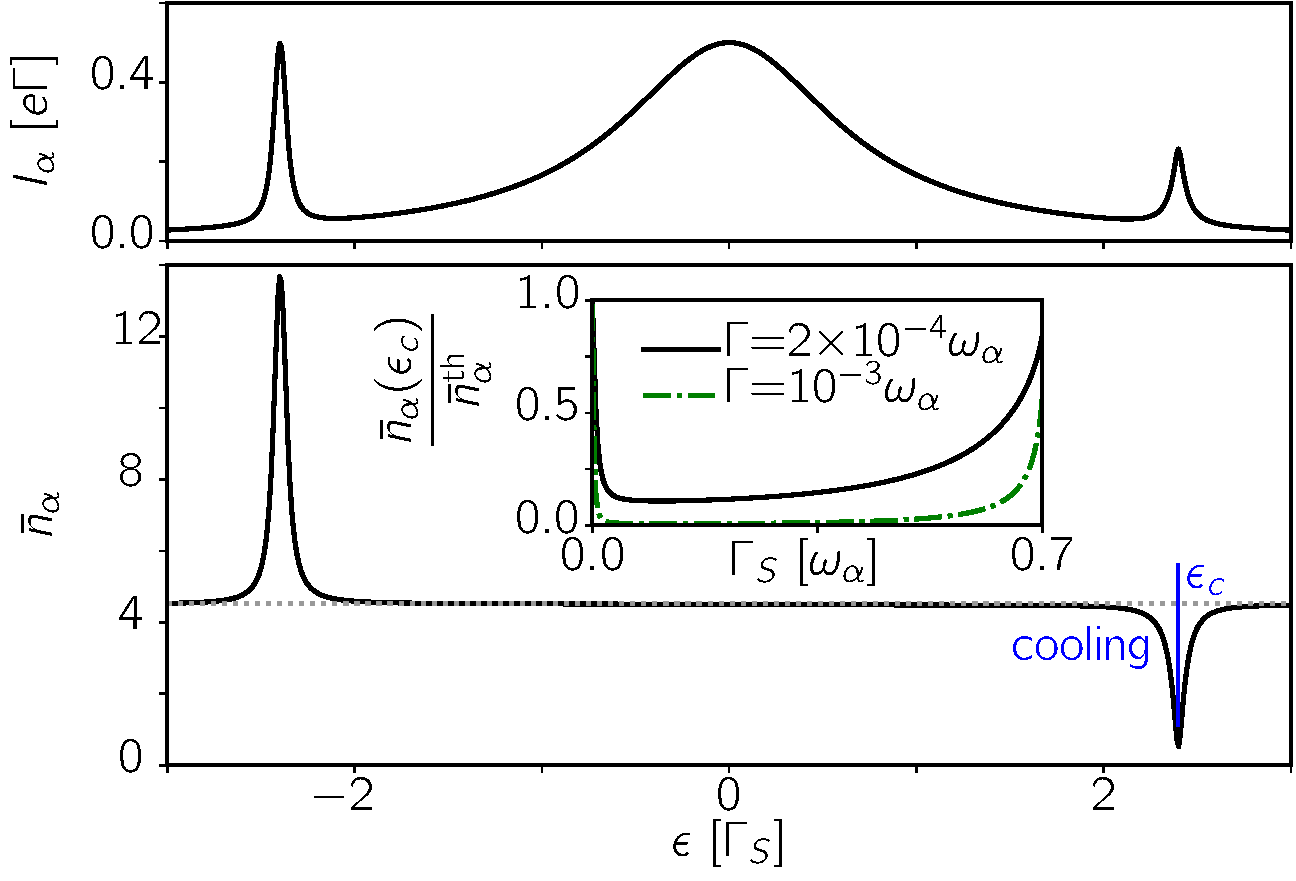
\includegraphics{Fig2.eps}}
\newlength\figurewidth
\newlength\figureheight
\settoheight\figureheight{\figure}
\settowidth\figurewidth{\figure}
\geometry{paperwidth=\figurewidth,paperheight=\figureheight,margin=0in}
\begin{document}
\fontsize{24}{28.8} \selectfont
        % String substitutions in EPS
		\psfrag{A}{(a)}
	\psfrag{B}{(b)}
	\psfrag{-2}[B][B]{\hspace{-1ex}$-2$}
		\psfrag{0}[B][B]{$0$}
		\psfrag{2}[B][B]{$2$}
		\psfrag{4}[B][B]{$4$}
		\psfrag{8}[B][B]{$8$}
		\psfrag{12}[B][B]{\hspace{1ex}$12$}
		\psfrag{0.0}[B][B]{$0.0$}
		\psfrag{0.4}[B][B]{$0.4$}
		\psfrag{0.5}[B][B]{$0.5$}
		\psfrag{0.7}[B][B]{$0.7$}
		\psfrag{1.0}[B][B]{$1.0$}
		\psfrag{cooling}{\textcolor{blue}{cooling}}
		\psfrag{epsCooling}{${\color{blue}\epsilon_{c}}$}
		\psfrag{rGN=0.2m}{$\Gamma{=}2{\times}10^{-4}\omega_\alpha$}
		\psfrag{rGN=1.0m}{$\Gamma{=}10^{-3}\omega_\alpha$}
		\psfrag{rT=0.0}{$k_B T = 0$}
		\psfrag{rT=5.0}{$k_B T = 5\omega_\alpha$}
		\psfrag{GSInwL}{$\Gamma_S$ [$\omega_\alpha$]}
		\psfrag{nLNorm}{$\dfrac{{\bar n}_\alpha(\epsilon_{c})}{{\bar n}_\alpha^{\rm th}}$}
		\psfrag{IL}[][]{$I_\alpha$ [$e\Gamma$]}
		\psfrag{nOscL}[][]{${\bar n}_\alpha$}
		\psfrag{eps}[B][c]{$\epsilon$ [$\Gamma_S$]}

        % Place the figure
        \figure
\end{document}
